\documentclass[12pt,twocolumn]{article}

% \usepackage{CormorantGaramond}
\usepackage{parskip}
\hyphenation{op-ti-mi-za-tion}
\usepackage{hologo}% to access the XeTeX logo via \hologo{XeLaTeX}
\usepackage{fontspec}
\setmainfont{EBGaramond-VariableFont_wght.ttf} % Times New Roman font
\usepackage{geometry}
\usepackage{graphicx}
\usepackage{lipsum} % For generating dummy text
\usepackage[english]{babel}
\usepackage{fancyhdr}
\usepackage{multicol}
\usepackage{xcolor}
\usepackage{csquotes}
\usepackage{enumitem}
\usepackage[style=ieee, backend=biber]{biblatex}
\usepackage[linesnumbered,ruled,vlined]{algorithm2e}
\addbibresource{reference.bib}
%\usepackage[style=authoryear]{biblatex}
\usepackage{soul}
% Define custom color for the abstract block
\definecolor{abstractcolor}{RGB}{240,240,240}
% Define header and footer
\pagestyle{fancy}
\fancyhf{} % Clear header and footer
\renewcommand{\headrulewidth}{0pt} % Remove header line
\renewcommand{\footrulewidth}{0.5pt} % Add footer line
\fancyfoot[C]{\thepage} % Page number in the center of the footer

\usepackage{algorithm}
\usepackage{algpseudocode}
\usepackage{amsmath}
\usepackage{forloop}
% Margins
\geometry{letterpaper, margin= 1.55cm, columnsep=25pt } % Adjust as needed

% Line spacing
\linespread{1.25}

\begin{document}

%  Main Page 1 
\begin{titlepage}
    \begin{center}
        \vspace*{1cm}
        
        {\fontspec{EBGaramond-Bold.ttf}\LARGE Ransomware Detection Application} \\
        \Large{Implementation of \\ {\fontspec{EBGaramond-SemiBold.ttf}Ransomware detection and mitigation using software-defined networking: The case of WannaCry}}
        
        \vspace{0.6cm}
        
        \Large by
        
        {\fontspec{EBGaramond-Bold.ttf}\Large Hemant Kumar} \\
        (Roll No. 20BCS100)
        
        \vspace{1cm}
        
        \Large Supervisor:
        
        {\fontspec{EBGaramond-Bold.ttf}\Large Dr. Neelam Dayal }\\
            (Assistant Professor) \\
        Computer Science and Engineering \\
        PDPM IIITDM Jabalpur
        
        \vspace{1cm}
        
        % External Supervisor(s):  
        
        % Name of External Supervisor \\
        % Company/Institute Address
        
        \vfill
        
        % Institute emblem
        
\includegraphics[width=30mm]{logo_college copy.png}
        
        \vspace{0.5cm}
        
        \Large{Computer Science and Engineering 
        \\ PDPM Indian Institute of Information Technology, Design and Manufacturing, Jabalpur}
        \\ (2024)
        
    \end{center}
\end{titlepage}
%  Main Page 1 Ends 


\begin{titlepage}
    \begin{center}
        \vspace*{1cm}
        
        {\fontspec{EnglishTowne.ttf} \LARGE Acknowledgement}
        
        \vspace{1.2cm}
        
        % Your acknowledgment paragraph goes here
       \large I would like to express my sincere gratitude to all the people who contributed in some way to the work described in this Project. Primarily I thanks to my respected supervisor, {\fontspec{EBGaramond-Bold.ttf}Dr. Neelam Dayal}, Assistant Professor in Computer Science and Engineering department, during my tenure of {\fontspec{EBGaramond-Bold.ttf}BTP}, she contributed to an enriching college experience by giving me intellectual freedom in my work, providing me inspiration and motivation, engaging me with new ideas, and demanding a high quality of work in all my endeavors. It was a matter of great felicity and privilege for me to work under his auspices. Additionally, I would like to thanks {\fontspec{EBGaramond-Bold.ttf}Dr. Abhishek Verma} (Assistant Professor), I.T Deptt. from the {\fontspec{EBGaramond-Bold.ttf}BabasahEB Bhimrao Ambedkar University, Lucknow} for their interest in my work, for extending their valuable time and support throughout my Project.

       I owe special thanks to my Project Partner {\fontspec{EBGaramond-Bold.ttf}Chaitanya Mandi, Roll-no: 20BCS062} for his support and suggestions that kept me motivated to accomplish my research work during my course duration.  I would like to thanks my all seniors, of the Computer Science and Engineering Department including the non-teaching staff with whom I got the opportunity to work in a healthy and joyful environment.

       Finally, I would like to acknowledge my beloved family members who supported me during my time here. I am really obliged for their constant love and support.
        % Add any additional acknowledgments here
        
        \vfill % Adjust the vertical space as needed
        
        \hrule % Add a horizontal line
        
        \vspace{1cm} % Adjust the vertical space after the line
        
        % Your name on the right-align
    \hfill {\fontspec{EBGaramond-Bold.ttf}Hemant Kumar}
        
        % \vfill % Fill the remaining vertical space
        
        % Institute emblem (if needed)
        
    \end{center}
\end{titlepage}

%  Main Page 1 Ends 


\begin{titlepage}
    \begin{center}
        \vspace*{1cm}
        
        {\fontspec{EnglishTowne.ttf}\LARGE Certificate}
        
        \vspace{1.2cm}
        
        % Your acknowledgment paragraph goes here
       \large This is to certify that the Report entitled, {\fontspec{EBGaramond-bold} "Ransomeware Detection Application"}, submitted by {\fontspec{EBGaramond-bold} Hemant Kumar, Roll No. 20BCS100} in partial fulfillment of the requirements for the award of {\fontspec{EBGaramond-bold} B.Tech Degree in Computer Science and Engineering}, at PDPM Indian Institute of Information Technology, Design and Manufacturing Jabalpur is an authentic work carried out by him under my supervision and guidance.
    
    
        To the best of my knowledge, the matter embodied in the thesis has not been submitted elsewhere to any other university/institute for the award of any other degree.
        % Add any additional acknowledgments here
        
        \vfill % Adjust the vertical space as needed

         
    \noindent
    \begin{tabular}{@{}ll@{}}
        {\fontspec{EBGaramond-Bold} Dr. Neelam Dayal} & \hfill {\fontspec{EBGaramond-Bold} {{2024-02-22}}} \\
        \large Assistant Professor & \\
        \parbox[t]{0.57\textwidth}{%
            Computer Science and Engineering Discipline, \\
            PDPM Indian Institute of Information Technology, Design and Manufacturing, Jabalpur, M.P, India-482005
        }
    \end{tabular}



       \vspace{2cm}
        
    \end{center}
\end{titlepage}

%  Main Page 1 Ends 

% Contents Starts Here

% Abstract
\twocolumn[

\hrule
   \begin{abstract}
\hrule

\vspace*{0.5 cm}
    % \lipsum[1] % Generate dummy abstract text
    {\fontspec{EBGaramond-Bold}Background:} Ransomware poses a severe threat to the security of digital assets, with a rising frequency of sophisticated attacks targeting individuals and organizations globally. The potential for significant financial and reputational damage underscores the urgent need for robust and proactive countermeasures. Traditional antivirus solutions often fall short in detecting evolving ransomware variants, necessitating the development of advanced detection applications.
    
    {\fontspec{EBGaramond-Bold}Aim:} The primary objective of this research is to design, implement, and evaluate a cutting-edge Ransomware Detection Application. Leveraging innovative techniques, including machine learning and behavioral analysis, our application aims to provide real-time detection and mitigation of ransomware threats. By enhancing the resilience of systems against emerging attack vectors, the goal is to fortify the cybersecurity posture of individuals and organizations in the face of evolving ransomware landscape.
    
    {\fontspec{EBGaramond-Bold}Conclusion:} The developed Ransomware Detection Application showcases promising results in effectively identifying and neutralizing ransomware threats. Through extensive testing and validation, our application demonstrates a high level of accuracy and efficiency in differentiating normal user behavior from malicious activities associated with ransomware attacks. The successful deployment of this solution contributes significantly to the ongoing efforts to secure digital environments against the menace of ransomware.
    
    {\fontspec{EBGaramond-Bold}Keywords:} Ransomware, Detection Application, Cybersecurity, Machine Learning, Behavioral Analysis, Threat Mitigation, Real-time Protection, Cyber Threats, Digital Security, Antivirus Solutions.
    
\end{abstract}

\vspace*{0.5 cm}
\hrule
\vspace*{0.8 cm}
]

% Abstract

% Introduction
\section{Introduction}

    In an era dominated by digital connectivity, the persistent threat of ransomware looms large, posing a formidable challenge to the security of individuals and organizations alike. Ransomware, a malicious software that encrypts or locks files and demands a ransom for their release, has evolved into a sophisticated and dynamic cyber threat. Understanding the nuances of ransomware is pivotal in developing effective countermeasures to safeguard against its pernicious impacts.

    Ransomware, at its core, is a form of cyber extortion wherein malicious actors leverage advanced encryption algorithms to restrict access to files or entire systems. The victim, often left with no recourse, is coerced into paying a ransom, typically in cryptocurrency, to obtain the decryption key. This nefarious practice has given rise to various types of ransomware, each exhibiting distinct characteristics and complexities.
    
    {\fontspec{EBGaramond-MediumItalic}Encrypting Ransomware:} This variant employs robust encryption algorithms, rendering files inaccessible until a ransom is paid. Notable examples include CryptoLocker and WannaCry.

    {\fontspec{EBGaramond-MediumItalic}Locker Ransomware:} Instead of encrypting files, locker ransomware locks users out of their systems, demanding payment for access restoration. Instances like the FBI virus and Winlocker fall into this category.

    {\fontspec{EBGaramond-MediumItalic}Scareware:} While not encrypting files, scareware falsely claims the presence of malware, tricking users into paying for non-existent security solutions.

    {\fontspec{EBGaramond-MediumItalic}Mobile Ransomware:} Targeting mobile devices, this variant demands payment for decrypting files or unlocking the device. Svpeng and Android Defender are prominent examples.
    
    {\fontspec{EBGaramond-MediumITalic}Doxware/Leakware:} This type of ransomware not only encrypts files but also threatens to release sensitive information to the public if the ransom is not paid. It adds a layer of extortion by leveraging the fear of data exposure.
    
    Ransomware works in several stages, first stage is infection in this ransomware typically gain the access to a system through phishing emails containing malicious attachments, compromised websites and exploiting vulnerabilities in software. Once executed it starts its malicious activities.Second stage is encryption, One common type of ransomware encrypts the victim's files using strong encryption algorithms. This renders the files inaccessible without the decryption key, which only the attacker possesses. After encrypting the files, the ransomware displays a ransom note informing the victim of the encryption and demanding payment, often in cryptocurrency like Bitcoin, Ethereum, or Monero. The note typically includes instructions on how to pay the ransom and obtain the decryption key. If the victim decides to pay the ransom, they follow the instructions provided in the ransom note to transfer the cryptocurrency to the attacker's wallet. However, there is no guarantee that paying the ransom will result in the decryption key being provided, and it may even encourage further attacks. In some cases, victims receive a decryption key after paying the ransom, allowing them to regain access to their files. However, there have been instances where the decryption key provided was faulty or the attacker disappeared after receiving payment, leaving the victim without recourse.
    
    Ransomware attacks can have severe consequences, including financial losses, data breaches, and disruption of operations for businesses and individuals.

% Requirement Analysis
\section{Requirement Analysis}

\subsection{\fontspec{EBGaramond-MediumItalic}Stakeholders' Requirements:}
    \begin{enumerate}[label=\arabic*.]
    \item End Users (Individuals and Organizations):
        \begin{itemize} 
            \item Detection Accuracy: Ensure the application accurately identifies and blocks known ransomware variants and detects novel ransomware behaviors. 
            \item Ease of Use: Provide a user-friendly interface with intuitive controls and minimal configuration requirements.
            \item Real-Time Protection: Offer real-time scanning and monitoring capabilities to detect and mitigate ransomware threats as they occur.
            \item Compatibility: Ensure compatibility with a wide range of operating systems, including Windows, macOS, and Linux, to accommodate diverse user environments.
        \end{itemize}

        \item Security Professionals:
        \begin{itemize}
            \item Customization Options: Allow for advanced configuration settings and customization options to tailor the application to specific security requirements and preferences.
            \item Integration with Existing Systems: Support integration with existing security infrastructure, such as endpoint protection platforms (EPPs) and security information and event management (SIEM) systems, for seamless threat detection and response.
            \item Reporting and Analysis: Provide comprehensive reporting and analysis features to track ransomware incidents, analyze attack patterns, and generate actionable insights for incident response and remediation.
        \end{itemize}
    \end{enumerate}

    
\subsection{\fontspec{EBGaramond-MediumItalic}Functional Requirements:}

\begin{enumerate}[label=\arabic*.]
    \item Ransomware Detection:
        \begin{itemize}
             \item Signature-Based Detection: Implement signature-based detection mechanisms to identify known ransomware variants based on predefined patterns or signatures.
            \item Behavior-Based Detection: Utilize behavior-based detection techniques to monitor system activity for suspicious behaviors indicative of ransomware, such as file encryption, unauthorized file access, and unusual network traffic.
            \item Machine Learning-Based Detection: Incorporate machine learning algorithms to analyze ransomware behavior patterns and automatically detect new, previously unseen ransomware threats.
        \end{itemize}

    \item Real-Time Protection:  
        \begin{itemize}
            \item Continuous Monitoring: Continuously monitor system activity in real-time to detect and respond to ransomware threats as they emerge.
            \item Immediate Response: Provide immediate response capabilities to block ransomware processes, quarantine infected files, and prevent further damage to the system.
        \end{itemize}

    \item Alerting and Notification:
        \begin{itemize}
            \item Alert Generation: Generate alerts and notifications to inform users and administrators of ransomware detections and potential security incidents.
            \item Severity Levels: Assign severity levels to ransomware incidents based on the level of risk and impact to facilitate prioritization and response.
        \end{itemize}
           
\end{enumerate}

\subsection{\fontspec{EBGaramond-MediumItalic}Non-Functional Requirements:}

\begin{enumerate}
    \item Performance:

        \begin{itemize}
            \item Low Resource Usage: Ensure the application operates efficiently with minimal impact on system performance and resource utilization.

            \item Scalability: Support scalability to accommodate varying workloads and environments, from individual users to large enterprises.
        \end{itemize}
    \item Reliability:
        \begin{itemize}
            \item High Availability: Maintain high availability and reliability to ensure uninterrupted protection against ransomware threats.

            \item Failover Mechanisms: Implement failover mechanisms and redundancy measures to minimize downtime and ensure continuous protection in the event of system failures or disruptions.
        \end{itemize}


    \item Security:
    \begin{itemize}
            \item Data Privacy: Ensure the confidentiality and integrity of sensitive data processed by the application, including threat intelligence, detection logs, and configuration settings.

            \item Secure Communication: Utilize secure communication protocols and encryption mechanisms to protect data transmitted between the application and external systems or services.
    \end{itemize}
\end{enumerate}

% Image Embed
\begin{figure*}[ht]
  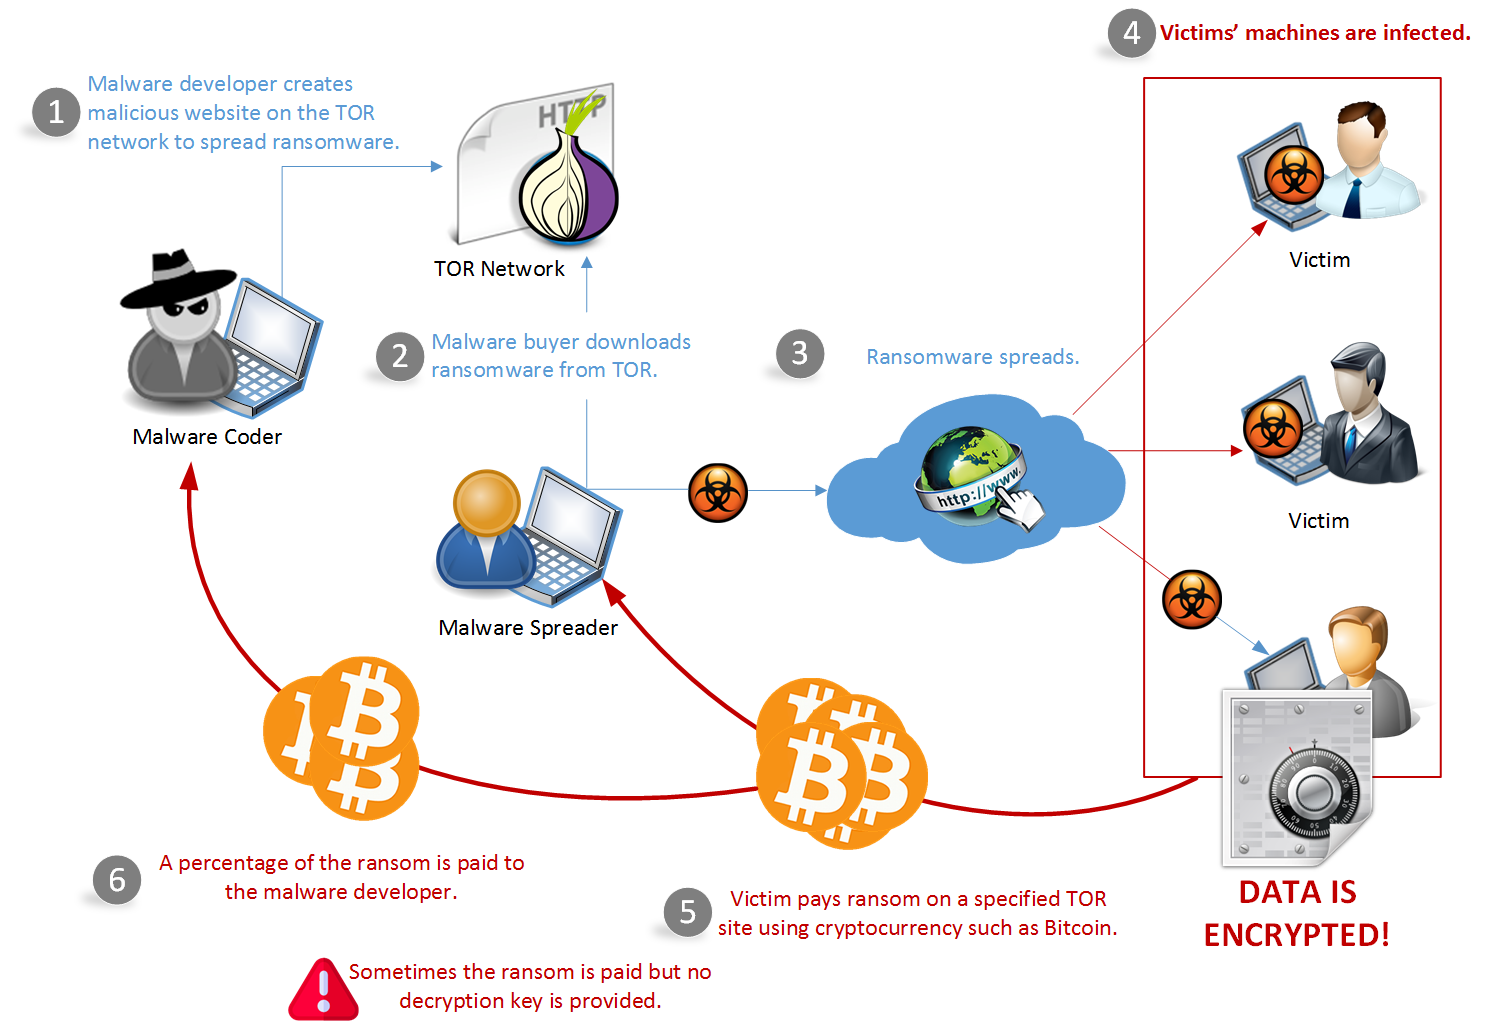
\includegraphics[width=\textwidth, height= 8 cm]{20180214-Free-Ransomware-1.png} % Replace example-image with your actual image file
  \caption{Generic working of Ransomware}
  \label{fig:my_label}
\end{figure*}

%
\vspace*{0.5 cm}

% Methodology
\section{Methodology}

In the fight against ransomware, a comprehensive approach involving various detection techniques is essential. The following sections detail the methodologies employed, each with its strengths and weaknesses.

We are trying to implement Ransomware Detection with differently approach, that no one might though about. In our detection Approach, we can develop some kind of algorithm and tactics which can scan, ransomware, and not only ransomware, but any kinds of malicious sect of code/ file, which can leads to execution of ransomware. \cite{AKBANOV2019111}

The execution of attacks on a node or within a network entails a systematic series of steps designed to optimize efficacy while minimizing the risk of detection. These steps encompass a structured approach to planning, reconnaissance, exploitation, and post-exploitation activities. Each phase is meticulously orchestrated to achieve specific objectives and maintain operational security. The methodology adheres to established principles of ethical hacking and penetration testing, ensuring that security vulnerabilities are identified and remediated effectively. Throughout this process, comprehensive documentation and reporting are maintained to facilitate remedial action and improve the overall security posture of the targeted system or network.

\subsection{Steps involved in process of Attack:}

\begin{enumerate}[label=\arabic*.]
    \item Infection:

    \begin{enumerate}[label=\alph*.]
        \item Delivery: Ransomware reaches a target system through various methods like phishing emails with malicious attachments, infected websites, RDP (Remote Desktop Protocol) vulnerabilities, or unpatched software.

        \item Initial Foothold: Once the ransomware gains access, it exploits vulnerabilities to establish a foothold on the system. This might involve creating new user accounts, disabling security software, or spreading laterally across the network.
        
    \end{enumerate}

    \item Encryption:

    \begin{enumerate}[label=\alph*.]
        \item File Targeting: The ransomware identifies and targets critical files and documents on the victim's device or network. This could include financial records, personal data, business documents, or system files.

        \item Encryption Process: Using strong encryption algorithms, the ransomware encrypts the targeted files, making them inaccessible to the victim. This process might vary depending on the specific ransomware strain.

        \item Encryption Key Generation: During encryption, the ransomware creates a unique decryption key for each victim. This key is essential for regaining access to the encrypted files. However, the attackers keep this key for themselves.
        
    \end{enumerate}

    \item Ransom Demand:

        Ransom Note: The ransomware displays a ransom note on the victim's screen. This note explains the situation, highlights the urgency, and outlines the attacker's demands. It typically includes instructions on how to pay the ransom, often in cryptocurrency like Bitcoin, due to its anonymity. The note might threaten to permanently delete backups, leak stolen data, or launch further attacks if the ransom isn't paid within a specific time frame.

        \item Verification (Hypothetical Scenario):

            \begin{enumerate}[label=\alph*.]
                \item Ransom Payment: If the victim chooses to pay (not recommended), they'd follow the attacker's instructions, which might involve sending cryptocurrency to a specific address.
    
                \item Verification (Unreliable): In an ideal scenario (which isn't guaranteed with cybercriminals), the attackers might verify the payment received.
            \end{enumerate}
        
        \item Decryption (Hypothetical Scenario):

            \begin{enumerate}[label=\alph*.]
                \item Decryptor Delivery (Unreliable): Again, assuming the attackers keep their word, they might provide a decryptor tool or the unique decryption key to the victim.

                \item Decryption Process: The victim would then use the decryptor or key to decrypt the compromised files and regain access.
            \end{enumerate}

\subsection{Safety Precautions and Measures:}
    \item Recovery (Recommended Approach):
        \begin{itemize}
            \item Isolate Infected Systems: Disconnect affected devices from the network to prevent further spread.

            \item Report the Attack: Inform law enforcement agencies and relevant authorities to assist with investigation and potential recovery efforts.

            \item Restore from Backups: If you have up-to-date backups, restore your critical data from a safe, isolated location.
    
            \item Remediate Vulnerabilities: Patch software vulnerabilities, update security software, and implement stronger access controls to prevent future attacks.
    
        \end{itemize}
    
\end{enumerate}

Incorporating a combination of these techniques provides a layered defense against ransomware, enhancing the likelihood of early detection and mitigation.

%
\section{Progress Update}

\subsection{Creation and Testing of Ransomware}

We\'ve crafted ransomware leveraging Python on a WindowsNT OS. Initially, we attempted to develop it in a Linux environment, but research revealed that most ransomware operates exclusively on Windows. Our build relies on essential packages like \hl{pywin32} \& \hl{pywin32-ctypes}, exclusively available for Windows systems.
\\
Our ransomware, inspired by WannaCry, is coded using Python and cryptography. Similar to the actual WannaCry ransomware, our version utilizes a Command and Control (CnC) approach. However, implementing CnC for key provision and payment retrieval presents challenges, requiring a dedicated server setup. As setting up servers posed significant obstacles, we opted not to include the CnC functionality. Additionally, while ransomware can be perilous if misused, our development was purely educational. To prevent any unintended consequences, we disabled its actual functionality. Nonetheless, even in this dormant state, Windows Defender still detects and removes it.

\subsection{Steganography and Creation of Trojan}

In our exploration of Steganography, we delved into concealing data within innocuous files to evade detection. Leveraging this technique, we embarked on creating a trojan by binding a malware executable with a JPG image using WinRAR\'s SFX features.
\\
To achieve this, we carefully encoded the malware executable within the pixels of the JPG image, ensuring it remained undetectable to casual observation. With WinRAR\'s SFX capabilities, we combined the concealed malware executable and the JPG image, creating a single self-extracting archive.
\\
Upon execution, the trojanized file presents itself innocuously as a typical JPG image. However, upon extraction, the malware executable is unleashed, potentially compromising the victim\'s system. This covert method of embedding malware within seemingly harmless files exemplifies the insidious nature of modern cyber threats.

\section{Distribution and Detection Phase}

In the Distribution and Detection Phase, our focus lies on executing the ransomware deployment strategy while ensuring effective detection measures are in place. To plant the ransomware on victim machines, we'll leverage a sophisticated network setup incorporating components like OpenFlow, OpenVSwitch, and an external controller. This setup enables dynamic network management and facilitates the orchestration of malicious activities. Through phishing campaigns and manual intrusion techniques, we'll exploit vulnerabilities in target systems to gain unauthorized access. Once inside the network, we'll utilize OpenFlow to manipulate network flows and route traffic to infected endpoints. OpenVSwitch will be instrumental in creating virtual network overlays, allowing for the seamless distribution of ransomware payloads while evading detection.

In parallel, stringent detection mechanisms will be implemented to identify and mitigate ransomware threats. Intrusion Detection Systems (IDS) will be deployed to monitor network traffic for suspicious behavior patterns indicative of ransomware activity. Additionally, anomaly detection algorithms will be employed to flag deviations from normal network behavior. Integration with external threat intelligence sources will enhance detection capabilities by providing real-time insights into emerging threats. By combining advanced network management tools with robust detection mechanisms, we aim to effectively distribute ransomware payloads while minimizing the risk of detection and containment by security defenses.

% Future Work

\section{Future Works}

In the Distribution and Detection Phase, our strategy accounts for two distinct scenarios: external and internal attacks on victim systems. In the external attack scenario, adversaries from outside the network aim to infiltrate and compromise victim machines. This may involve exploiting vulnerabilities in network perimeter defenses or conducting phishing campaigns to trick users into downloading and executing malicious payloads. Conversely, in the internal attack scenario, adversaries already within the network leverage insider access or compromised credentials to propagate ransomware to additional endpoints.
\\
To illustrate these scenarios, our network setup encompasses various components, including OpenFlow, OpenVSwitch, and an external controller. OpenFlow facilitates dynamic network control, allowing us to manipulate network flows and route traffic to targeted endpoints. OpenVSwitch enables the creation of virtual network overlays, facilitating the seamless distribution of ransomware payloads while evading detection. An external controller orchestrates these activities, providing centralized management and coordination of network operations.
\\
In the external attack scenario, adversaries exploit vulnerabilities in network defenses to gain unauthorized access. Phishing campaigns may lure unsuspecting users to click on malicious links or download infected attachments, enabling adversaries to plant ransomware on victim machines. Meanwhile, in the internal attack scenario, adversaries leverage insider access or compromised credentials to move laterally within the network, infecting additional endpoints with ransomware payloads.
\\
To visually represent these scenarios, we'll provide networking diagrams illustrating the network topology, including the placement of components like OpenFlow switches, OpenVSwitch instances, and the external controller. Additionally, we'll embed images showcasing the two attack scenarios, highlighting the pathways through which ransomware is distributed to victim machines. By presenting these visual aids, we aim to provide a comprehensive understanding of our distribution and detection strategy in both external and internal attack scenarios.

\begin{figure}[htbp]
    \centering
    \includegraphics[width=0.5\textwidth]{example-image.jpg}
    \caption{Example Image}
    \label{fig:example}
\end{figure}



\begin{figure}[htbp]
    \centering
    \includegraphics[width=0.5\textwidth]{example-image.jpg}
    \caption{Example Image}
    \label{fig:example}
\end{figure}


% Conclusion
\section{Conclusion}
Work is going on, on final Report it will be disclosed.
since our Detection and Mitigation System is not completed yet.
% \begin{algorithm}
% \caption{AES CBC Encrypt}
% \begin{algorithmic}
% \Function{AES\_CBC\_Encrypt}{$\text{plaintext}, \text{key}, \text{iv}$}
%   \State $ \text{// Divide plaintext into 128-bit blocks} $
%   \State $ \text{blocks} \gets \text{splitBlocks(plaintext, 128)} $
%   \State $ \text{previousCiphertext} \gets \text{iv} $
%   \State $ \text{// Generate round keys for AES} $
%   \State $ \text{roundKeys} \gets \text{getRoundKeys(key)} $
%   \newcounter{BlockIndex}
%   \setcounter{BlockIndex}{0}
%   \loop
%     \ifnum\value{BlockIndex}<\numexpr\lengthof{blocks}\relax
%       \State $ \text{// XOR plaintext block with previous ciphertext} $
%       \State $ \text{xoredBlock} \gets \text{xor(blocks[\arabic{BlockIndex}], previousCiphertext)} $
%       \State $ \text{// Encrypt xored block using AES} $
%       \State $ \text{encryptedBlock} \gets \text{AES\_Encrypt(xoredBlock, roundKeys)} $
%       \State $ \text{// Update previous ciphertext for next block} $
%       \State $ \text{previousCiphertext} \gets \text{encryptedBlock} $
%       \stepcounter{BlockIndex}
%   \repeat
%   \State $ \text{// Combine encrypted blocks as ciphertext} $
%   \State $ \text{ciphertext} \gets \text{combineBlocks(encryptedBlock)} $
%   \State \Return $\text{ciphertext}$
% \EndFunction
% \end{algorithmic}
% \end{algorithm}


% \begin{algorithm}
% \caption{AES CBC Decrypt}
% \begin{algorithmic}
% \Function{AES\_CBC\_Decrypt}{$\text{ciphertext}, \text{key}, \text{iv}$}
%   \State $ \text{// Split ciphertext into 128-bit blocks} $
%   \State $ \text{blocks} \gets \text{splitBlocks(ciphertext, 128)} $
%   \State $ \text{// Initialize previous ciphertext with IV} $
%   \State $ \text{previousCiphertext} \gets \text{iv} $
%   \State $ \text{// Loop through each ciphertext block} $
%   \State $ \text{decryptedBlocks} \gets [] $
%   \newcounter{BlockIndex}
%   \setcounter{BlockIndex}{0}
%   \loop
%     \ifnum\value{BlockIndex}<\numexpr\lengthof{blocks}\relax
%       \State $ \text{// Decrypt ciphertext block using AES} $
%       \State $ \text{decryptedBlock} \gets \text{AES\_Decrypt(blocks[\arabic{BlockIndex}], roundKeys)} $
%       \State $ \text{// XOR decrypted block with previous ciphertext} $
%       \State $ \text{xoredBlock} \gets \text{xor(decryptedBlock, previousCiphertext)} $
%       \State $ \text{// Update previous ciphertext for next block} $
%       \State $ \text{previousCiphertext} \gets \text{blocks[\arabic{BlockIndex}]} $
%       \State $ \text{// Append xored block to decrypted blocks} $
%       \State $ \text{append(decryptedBlocks, xoredBlock)} $
%       \stepcounter{BlockIndex}
%   \repeat
%   \State $ \text{// Combine decrypted blocks as plaintext} $
%   \State $ \text{plaintext} \gets \text{combineBlocks(decryptedBlocks)} $
%   \State \Return $\text{plaintext}$
% \EndFunction
% \end{algorithmic}
% \end{algorithm}


\twocolumn[
    \printbibliography
]
\end{document}
